\section{Conventions de signe}

	Il nous faut, hélas, une fois de plus convenir de quelques notations graphiques et de signe avant de s’attaquer au corps du sujet.

	Dans ce chapitre, nous étudierons tant des machines thermiques à l’intérieur desquelles une quantité fixe de fluide est captive (mieux étudiées à l’aide d’un système fermé, \textit{cf.} le \coursdeuxshort), que des machines à l’intérieur desquelles le fluide circule en continu (mieux étudiées à l’aide d’un système ouvert, \textit{cf.} le \courstroisshort).

	Nos conventions graphiques pour représenter ces machines sont décrites en figures~\ref{fig_conventions_graphiques_flèches_petites} et~\ref{fig_conventions_graphiques_flèches_larges}.

	\begin{figure}
		\begin{center}
			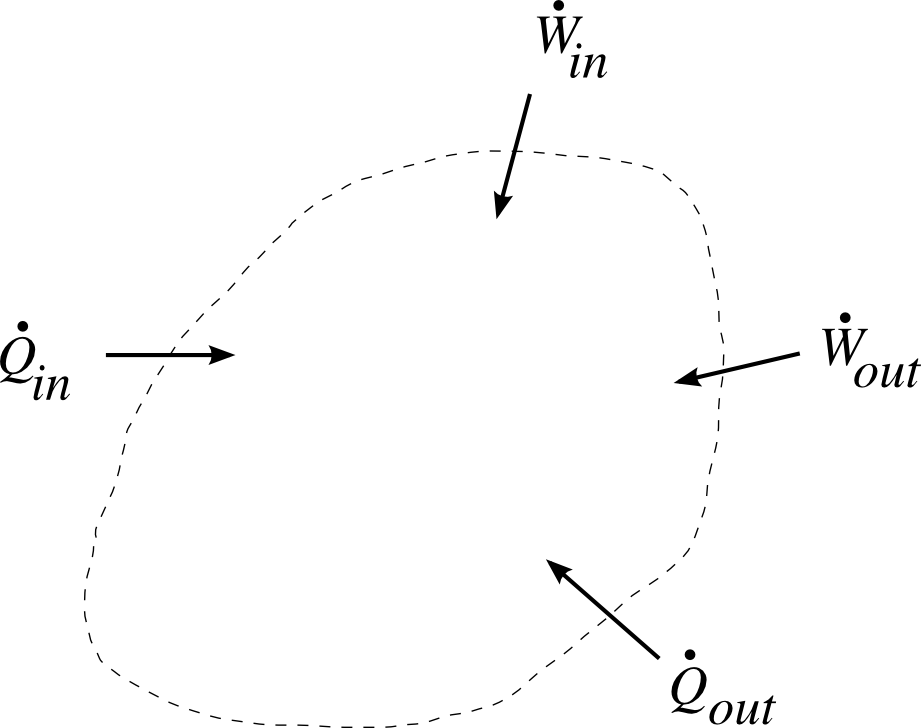
\includegraphics[width=8cm]{images/cours6-img3.png}
		\end{center}
		\caption{Convention graphique utilisée jusqu’à présent.
			La quantité de masse à l’intérieur de la machine est fixe, et elle fonctionne de façon continue.
			Nous avons $\dot{W}_\text{in} + \dot{W}_\text{out} + \dot{Q}_\text{in} + \dot{Q}_\text{out} = 0$}
		\label{fig_conventions_graphiques_flèches_petites}
	\end{figure}

	\begin{figure}
		\begin{center}
			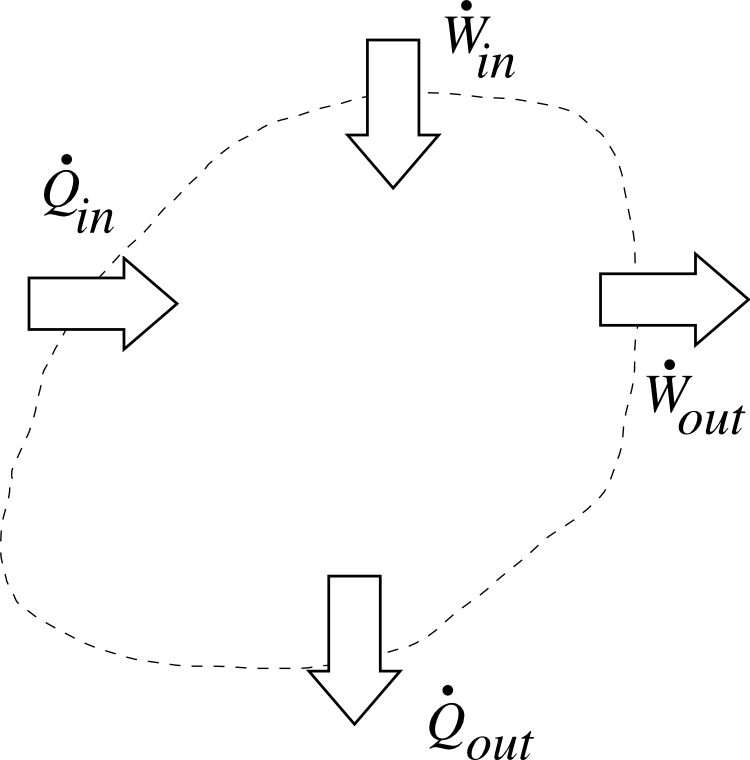
\includegraphics[width=8cm]{images/cours6-img4.png}
		\end{center}
		\supercaption{Nouvelle convention graphique.
			\textbf{Les larges flèches blanches indiquent le sens physique des transferts.}\\
			Par exemple, $\dot{W}_\text{out}$ étant négatif (car sortant), il est représenté par une large flèche sortante. Cette convention est plus intuitive pour décrire le fonctionnement des machines, mais également moins commode pour quantifier mathématiquement les transferts.}{}
		\label{fig_conventions_graphiques_flèches_larges}
	\end{figure}

	\clearfloats
	La somme du travail reçu et fourni par une machine est nommé le \vocab{travail net}\footnote{Attention, il est aisé de confondre le travail net (en anglais, \vocabe{net work}) avec le \vocabe{travail brut} (\vocabe{gross work}), soit $\dot{W}_\text{brut} \equiv |\dot{W}_\text{out}|$). Le travail net peut être positif ou négatif, en fonction du type de machine.}. Le concept est illustré en \cref{fig_conventions_graphiques_travail_net}.

	\begin{IEEEeqnarray}{rCl}
		W_\text{net} 			& \equiv & W_\text{in} + W_\text{out} 					\nonumber \\
		\dot{W}_\text{net} 	& \equiv & \dot{W}_\text{in} + \dot{W}_\text{out} 	\nonumber \\
		w_\text{net} 			& \equiv & w_\text{in} + w_\text{out}
	\label{def_travail_net}
	\end{IEEEeqnarray}

	\begin{figure}
		\begin{center}
			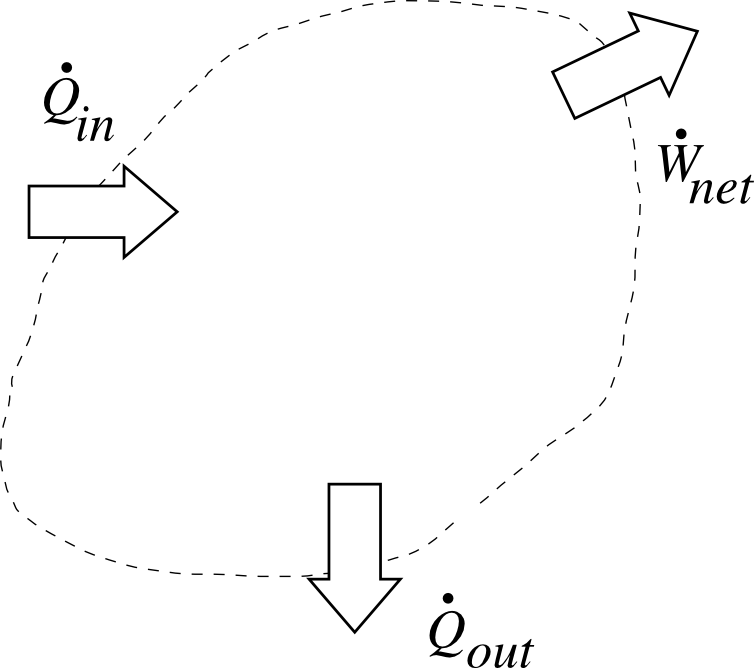
\includegraphics[width=8cm]{images/cours6-img5.png}
		\end{center}
		\caption{Les transferts de la \cref{fig_conventions_graphiques_flèches_larges} représentés différemment. Le travail rentrant $\dot W_\text{in}$ et le travail sortant $\dot W_\text{out}$ sont regroupés en un seul transfert, le travail net~$\dot W_\text{net}$.}
		\label{fig_conventions_graphiques_travail_net}
	\end{figure}

	On définit la \vocab{chaleur nette} de la même façon :
	\begin{IEEEeqnarray}{rCl}
		Q_\text{net} 			& \equiv & Q_\text{in} + Q_\text{out}	 				\nonumber \\
		\dot{Q}_\text{net} 	& \equiv & \dot{Q}_\text{in} + \dot{Q}_\text{out}	\nonumber \\
		q_\text{net} 	& \equiv & q_\text{in} + q_\text{out}
	\end{IEEEeqnarray}

	Ainsi, par exemple, un moteur automobile reçoit une chaleur nette positive et produit un travail net négatif.



\section{Transformer chaleur et travail}

	\subsection{Construire des cycles thermodynamiques}

		Si nous voulons qu’une machine fonctionne en continu, il faut qu’elle ramène le fluide qu’elle contient dans l’état où il était au début de son fonctionnement.

		Par exemple, il est aisé de refroidir une pièce avec une bouteille d’air comprimé (il suffit de le laisser travailler dans une détente pour que sa température chute) ; mais si nous voulons refroidir la pièce en continu, alors il nous faut aussi tenir compte de l’énergie nécessaire pour \textit{ramener} l’air dans la bouteille, à sa température initiale, à la fin du processus.

		Lorsque le fluide est ramené à son état initial (même température, même pression, même énergie interne), on dit qu’il a parcouru un cycle thermodynamique complet (\S\ref{ch_premier_principe_sf}).
		Tous les cycles ne sont pas équivalents. Nous allons assembler différentes évolutions pour les construire.


	\subsection{Produire un travail à partir de chaleur}
	\label{ch_principe_fonctionnement_moteur}

		Le raisonnement à l’origine du fonctionnement de n’importe quel moteur est assez simple. Lorsque l’on chauffe un fluide, sa pression et son volume ont tendance à augmenter ; on peut exploiter cela en lui faisant fournir un travail. 

		Avant de ramener le fluide à son volume initial, on le refroidit. Ainsi, on dépense moins de travail au chemin retour que l’on en a obtenu à l’aller. L’ensemble aura donc \emph{produit} du travail et absorbé (plus exactement, \emph{transformé}) de la chaleur.

		Il existe de multiples façons de faire évoluer un fluide pour transformer de la chaleur en travail, mais  toutes comportent quatre transferts énergétiques, comme représenté en figures~\ref{fig_cycle_thermodynamique_du_moteur_so} et~\ref{fig_cycle_thermodynamique_du_moteur_sf}. En fonction des contraintes technologiques et pratiques, certains de ces transferts peuvent être effectués simultanément.

		\begin{figure}
			\begin{center}
				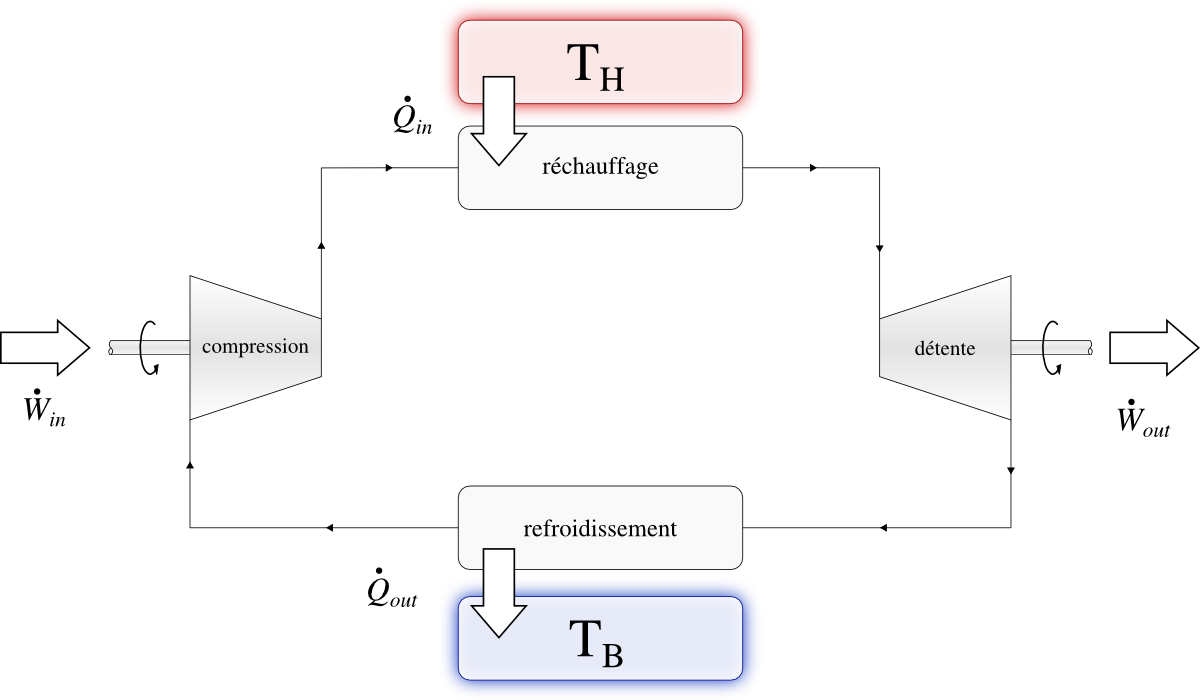
\includegraphics[width=\textwidth]{images/mot_so_1.png}
			\end{center}
			\caption{Cycle thermodynamique moteur, avec un circuit continu.
		La somme nette du travail (soit	$\dot{W}_\text{in} + \dot{W}_\text{out}$) est négative, c’est-à-dire que le fluide fournit une puissance $\dot{W}_\text{net}$ à l’extérieur..}
			\label{fig_cycle_thermodynamique_du_moteur_so}
		\end{figure}

		\begin{figure}
			\begin{center}
				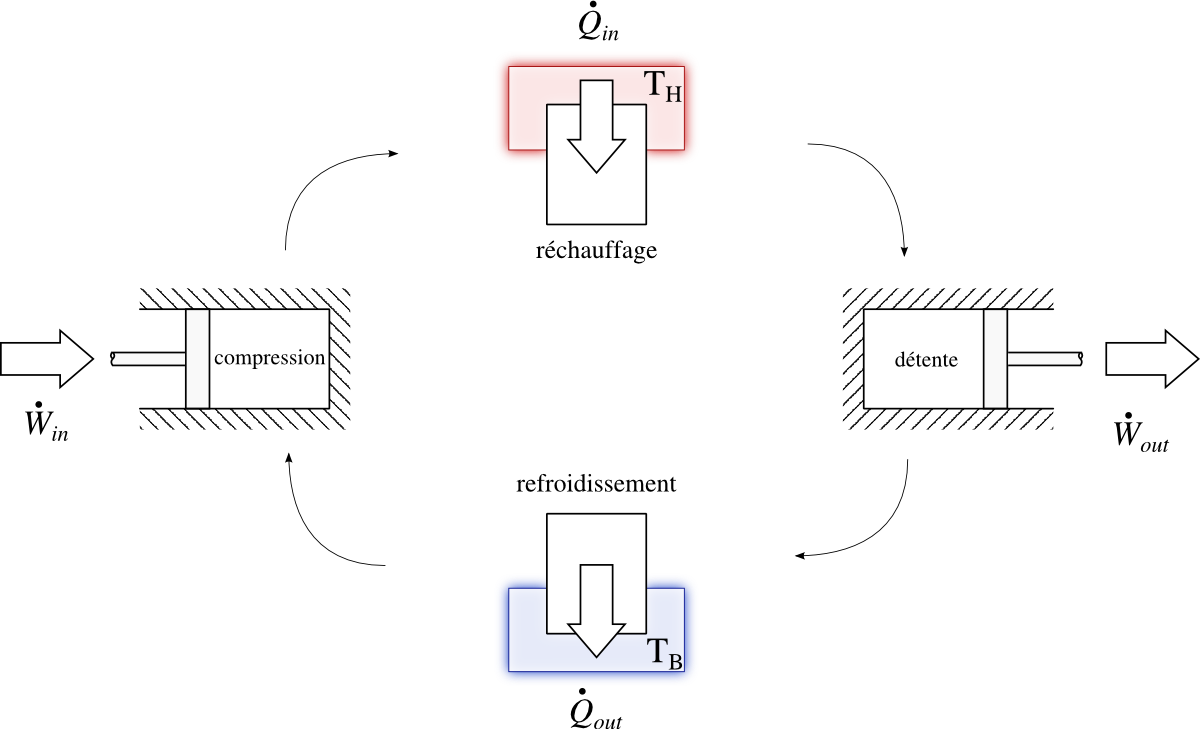
\includegraphics[width=\textwidth]{images/mot_sf_1.png}
			\end{center}
			\caption{Cycle thermodynamique moteur avec quatre évolutions successives.}
			\label{fig_cycle_thermodynamique_du_moteur_sf}
		\end{figure}

		La machine requiert un investissement extérieur sous forme de travail, $\dot{W}_\text{in}$~, pour la compression ; elle fournira, sous forme de travail également, une puissance $\dot{W}_\text{out}$ plus grande, lors de la détente.

		Il est bien sûr possible de relier mécaniquement les sections consommant et fournissant de l’énergie, comme représenté en figures~\ref{fig_cycle_thermodynamique_du_moteur_axe_so} et~\ref{fig_cycle_thermodynamique_du_moteur_axe_sf}. L’ensemble fournit alors directement une puissance nette $\dot{W}_\text{net}$ .

		\begin{figure}
			\begin{center}
				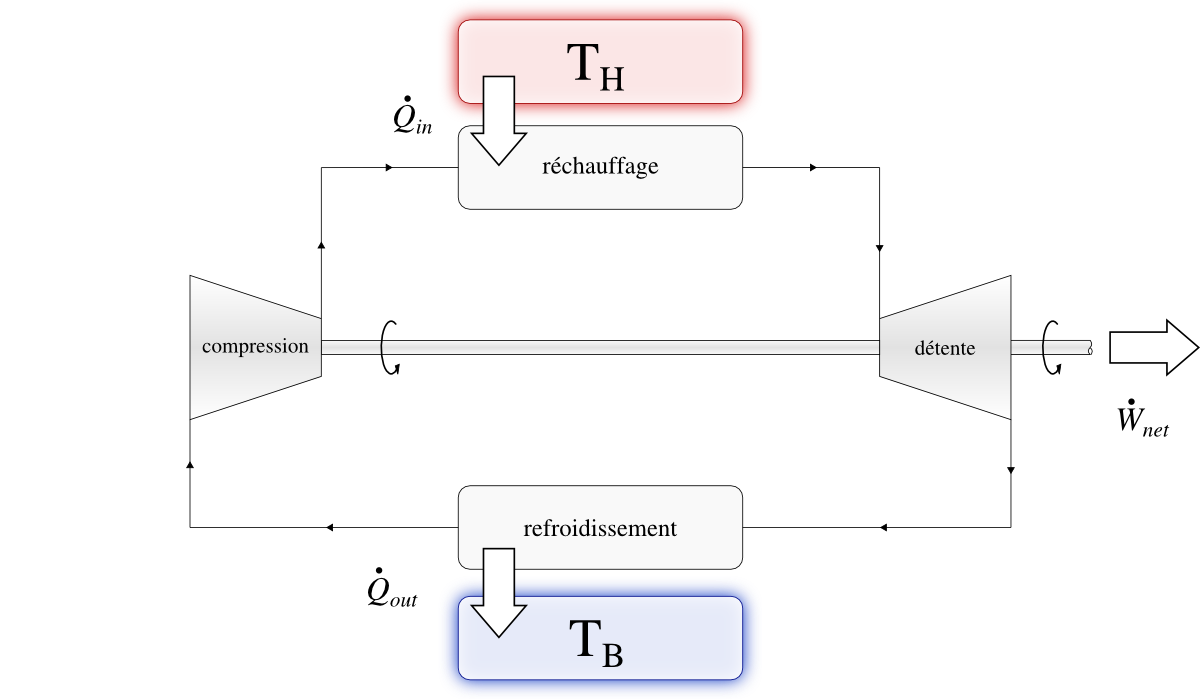
\includegraphics[width=\textwidth]{images/mot_so_2.png}
			\end{center}
			\caption{Cycle thermodynamique moteur, pour lequel le compresseur et la turbine sont reliés mécaniquement.
		La somme nette du travail (soit	$\dot{W}_\text{in} + \dot{W}_\text{out}$) est négative, c’est-à-dire que le fluide fournit une puissance $\dot{W}_\text{net}$ à l’extérieur.}
			\label{fig_cycle_thermodynamique_du_moteur_axe_so}
		\end{figure}

		\begin{figure}
			\begin{center}
				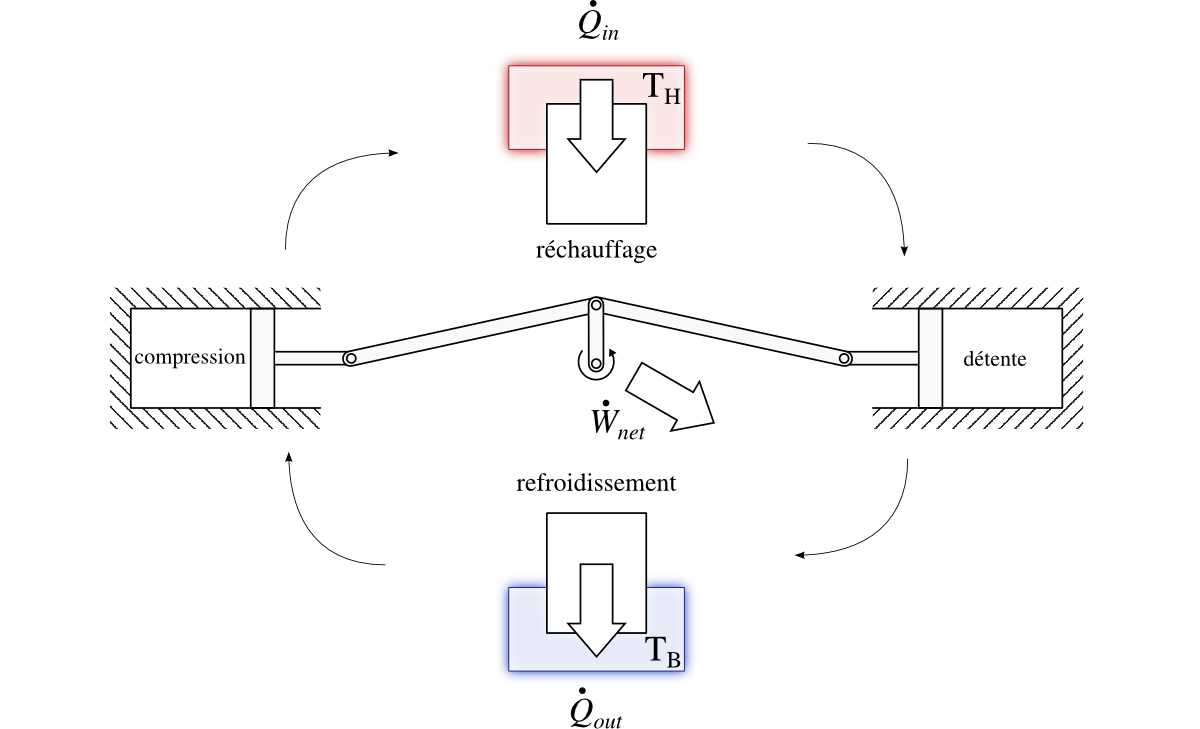
\includegraphics[width=\textwidth]{images/mot_sf_2.png}
			\end{center}
			\caption{Dans le moteur de la \cref{fig_cycle_thermodynamique_du_moteur_sf}, on peut relier mécaniquement la phase de compression et de détente, comme schématisé ici.}
			\label{fig_cycle_thermodynamique_du_moteur_axe_sf}
		\end{figure}


		En fonction des applications, certaines modifications sont apportées, par exemple :

		\begin{itemize}
			\item Dans un moteur à explosion, le cycle n’est pas effectué de façon continue mais par brèves évolutions successives ;
			\item La plupart des moteurs à air ne contiennent pas de «~refroidisseur~» proprement dit. 
			En effet, l’air étant disponible en abondance, il est plus simple de le rejeter dans l’atmosphère plutôt que de le laisser refroidir à l’intérieur du moteur\footnote{On pourra aussi mentionner que cela permet de ré-alimenter les cylindres avec de l’air oxygéné et sans déchets de combustion.}. 
			Le refroidissement a alors lieu en dehors du moteur physique. Le moteur perd de la chaleur avec l’air qu’il rejette ; cette perte est quantifiée exactement comme si on utilisait un refroidisseur interne\footnote{En termes thermodynamiques, on pourrait dire que l’atmosphère fait partie du moteur : elle ramène le fluide à son état initial en le refroidissant à pression constante.}\nolinebreak.
		\end{itemize}


	\subsection{Extraire de la chaleur avec du travail}
	\label{ch_principe_fonctionnement_réfrigérateur}

			Lorsque l’on fournit du travail à un fluide, sa température augmente,\footnote{C’est strictement vrai pour un gaz parfait. Comme nous l’avons vu dans le \courscinq, les liquides/vapeurs suivent aussi cette tendance mais connaissent une phase à température constante entre leurs points de saturation.} et il peut ainsi fournir de la chaleur à un corps qui était initialement plus «~chaud~» que lui.

			À l’inverse, lorsque l’on détend un fluide, sa température baisse,\footnote{La même remarque s’applique ici.} et il peut ainsi capter de la chaleur à un corps qui était initialement plus «~froid~» que lui.

			Lorsque ces étapes sont combinées en un cycle, nous obtenons le principe de fonctionnement d’un \vocab{réfrigérateur} : on \emph{extrait de la chaleur de l’intérieur} d’un récipient (basse température) et on la rejette à l’extérieur (à plus haute température). Le fonctionnement d’un réfrigérateur est décrit en figures~\ref{fig_principe_du_réfrigérateur_so} et~\ref{fig_principe_du_réfrigérateur_sf}.

			\begin{figure}
				\begin{center}
					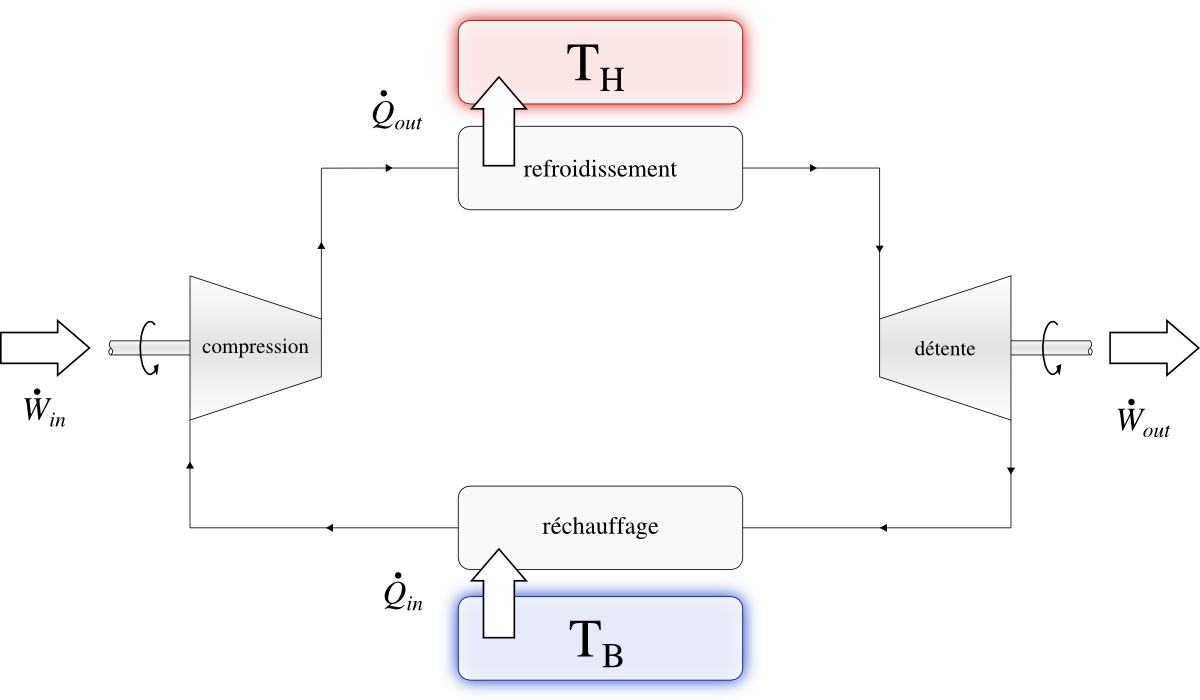
\includegraphics[width=\textwidth]{images/tp_so_1.png}
				\end{center}
				\supercaption{Cycle thermodynamique de refroidissement en cycle continu.\\
			Le travail net $\dot{W}_\text{net}$ est positif, c’est-à-dire que la machine doit être alimentée en travail par l’extérieur. De la chaleur $\dot{Q}_\text{in}$ est captée du corps «~froid~» à température~$T_B$, et de la chaleur $\dot{Q}_\text{out}$ est transmise au corps «~chaud~» (à température~$T_H$).}{}
				\label{fig_principe_du_réfrigérateur_so}
			\end{figure}

			\begin{figure}
				\begin{center}
					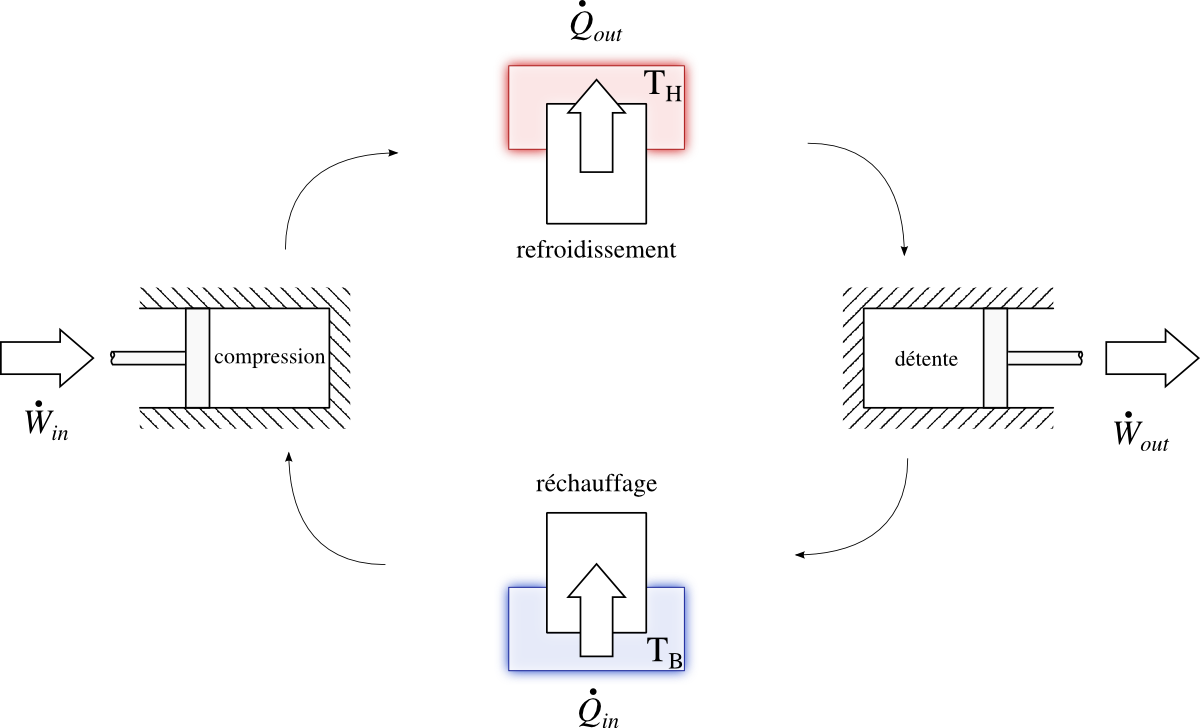
\includegraphics[width=\textwidth]{images/tp_sf.png}
				\end{center}
				\caption{Cycle thermodynamique de refroidissement en évolutions successives.}
				\label{fig_principe_du_réfrigérateur_sf}
			\end{figure}

			On peut aussi positionner la machine différemment. La chaleur est alors \emph{extraite de l’extérieur} (milieu à basse température) d’un bâtiment, et rejetée à l’intérieur de l’habitation (milieu à plus haute température). C’est le principe de la \vocab{pompe à chaleur}, que l’on appelle parfois \vocab{thermopompe}.\\
			On voit qu’une pompe à chaleur n’est rien de plus qu’un réfrigérateur positionné de sorte qu’il «~refroidisse l’extérieur~».

			\clearfloats
			En pratique dans les systèmes de réfrigération, on ne cherche pas toujours à produire un travail dans la phase de détente. Il est en effet souvent plus économique d’utiliser une simple soupape que d’extraire et acheminer du travail mécanique au travers de la machine.

			Cette soupape, en termes thermodynamiques, permet d’effectuer une détente irréversible, augmentant le volume et baissant la pression sans extraire de travail. Dans le cas d’un gaz parfait, cela n’aura aucun effet sur la température
				\footnote{Revoir à ce propos le principe de Joule étudié en section \S\ref{ch_principe_de_joule}}%
			(et donc aucun intérêt pratique) ; mais pour les mélanges liquide-vapeur, c’est un moyen technologiquement simple de faire chuter la température. Cette modification est décrite en \cref{fig_principe_du_réfrigérateur_soupape}.

			\begin{figure}
				\begin{center}
					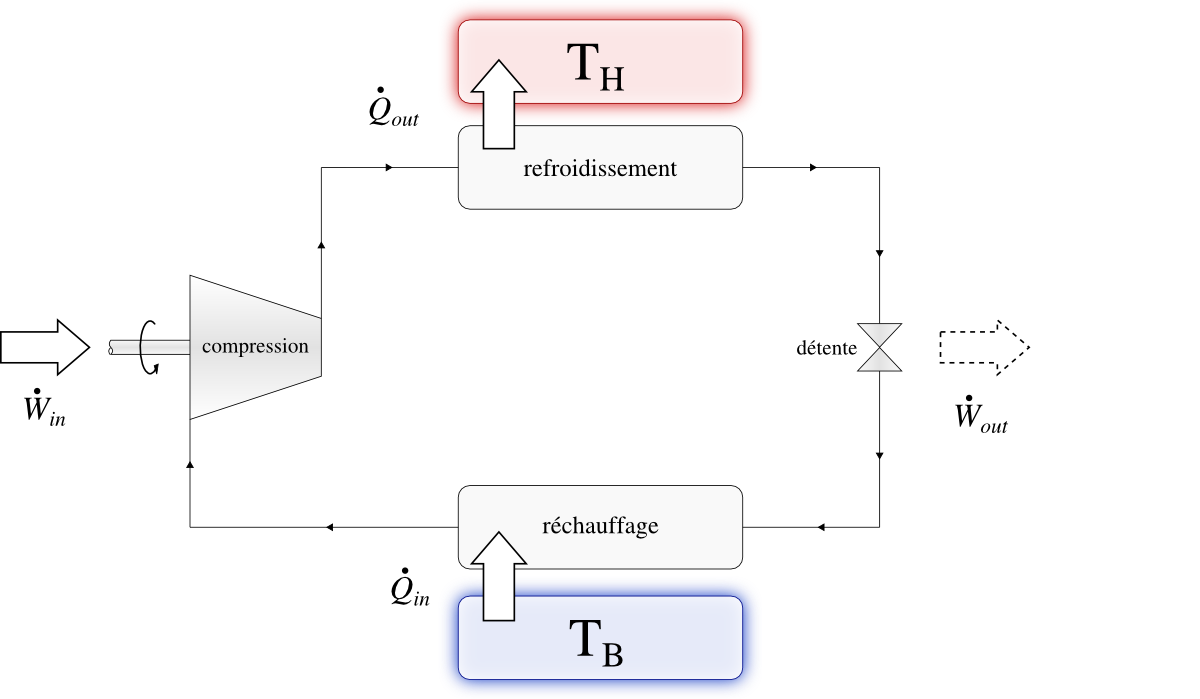
\includegraphics[width=\textwidth]{images/tp_so_2.png}
				\end{center}
				\caption{Cycle de refroidissement modifié. 
			Dans le cas de mélanges liquide-vapeur, il est possible de se dispenser d’extraire du travail lors de la détente. L’utilisation d’une simple soupape suffit pour faire baisser la température du fluide.}
				\label{fig_principe_du_réfrigérateur_soupape}
			\end{figure}





\section{Rendement des cycles}

		Le \vocab{rendement} d’une machine thermique compare le transfert ou la transformation utile qu’elle effectue, avec le coût énergétique qu’elle engendre. Nous retiendrons la définition de principe suivante :
		\begin{equation}
			\eta  \equiv  \left| \frac{\text{transfert utile}}{\text{dépense énergétique}} \right|
			\label{def_efficacité_machines_thermiques}
		\end{equation}

		Pour chacun des trois types de machines thermiques, nous allons définir et quantifier ce «~transfert utile~» et cette «~dépense énergétique~».



		\subsection{Rendement d’un moteur}
		\label{ch_rendement_moteur}

			La fonction d’un moteur thermique standard, comme ceux que l’on trouve à bord des automobiles ou dans les centrales électriques, est de produire du travail, c’est-à-dire une quantité $\dot{W}_\text{net}$ négative (\cref{fig_transferts_moteur}). La dépense engendrée pour générer ce travail est la chaleur qu’il reçoit, c’est-à-dire la quantité $\dot{Q}_\text{in}$ (provenant usuellement de la combustion de carburant ou de la fission de noyaux atomiques).

			\begin{figure}
				\begin{center}
					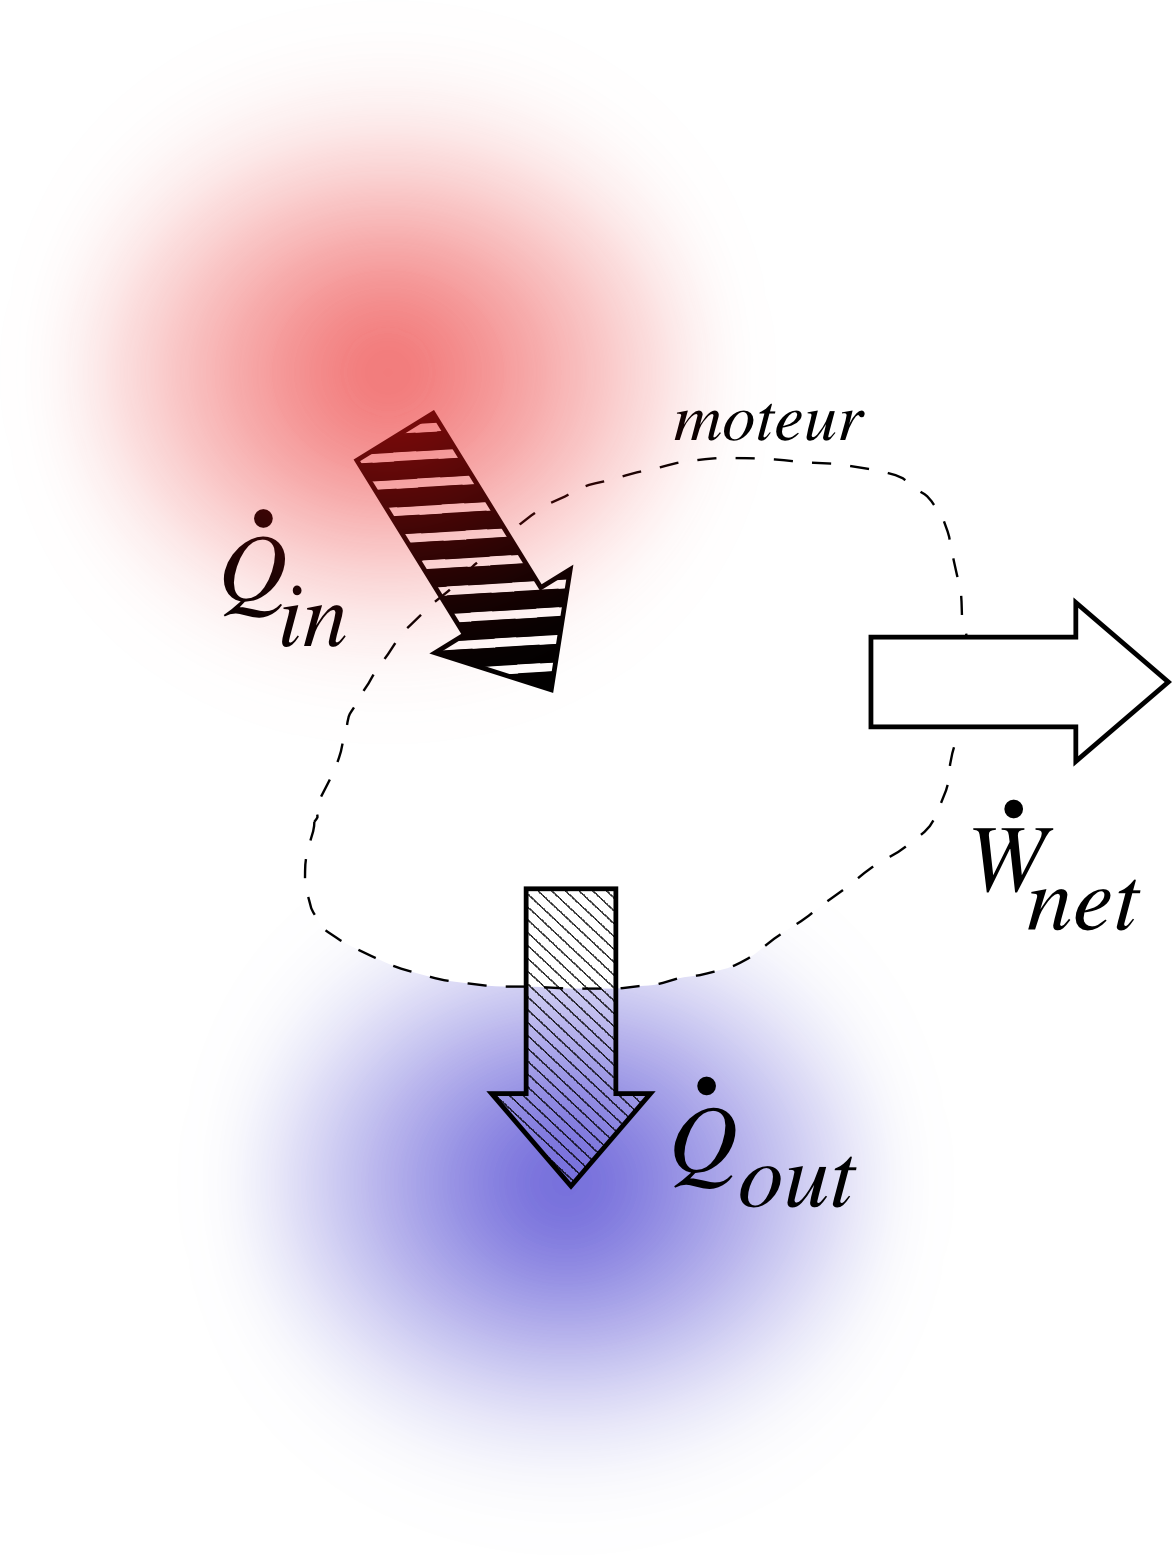
\includegraphics[height=10cm]{images/eff_moteur.png}
				\end{center}
				\caption{Schématisation d’un moteur standard.
			On souhaite obtenir un grand transfert $\dot{W}_\text{net}$  (résultat) à partir du transfert $\dot{Q}_\text{in}$ (coût). 
			Le rejet $\dot{Q}_\text{out}$ est indésirable.}
				\label{fig_transferts_moteur}
			\end{figure}

			D’après la définition~\ref{def_efficacité_machines_thermiques} le rendement du moteur thermique est donc :
			\begin{equation}
				\eta_\text{moteur} \equiv \left| \frac{\dot{W}_\text{net}}{\dot{Q}_\text{in}} \right|
				\label{def_rendement_moteur}
			\end{equation}

			\begin{anexample}
			Un moteur automobile reçoit une puissance de~\SI{100}{\kilo\watt} sous forme de chaleur issue de la combustion d’essence ; il fournit \SI{55}{\kilo\watt} sous forme de travail à l’arbre de transmission. Quel est son rendement ?
			
			\begin{answer}
				Le rendement est de $\eta_\text{moteur} = \left| \frac{\dot{W}_\text{net}}{\dot{Q}_\text{in}} \right| = \left| \frac{\num{-55e3}}{\num{+100e3}} \right| = \num{0,55} = \SI{55}{\percent}$. 
					\begin{remark} Ce moteur effectue un rejet $\dot{Q}_\text{out} = -\dot{W}_\text{net} - \dot{Q}_\text{in} = -(\num{-55e3}) - \num{100e3}= \SI{-45}{\kilo\watt}$. Cette chaleur est usuellement évacuée par le pot d’échappement.\end{remark}
					\begin{remark} On se doute bien qu’il faudra toujours fournir au moins autant de chaleur $\dot{Q}_\text{in}$ que le moteur ne fournit de travail $\dot{W}_\text{net}$ ; le rendement d’un moteur sera donc toujours nécessairement inférieur à~\num{1}.\end{remark}
			\end{answer}
		\end{anexample}

			Par exemple, un moteur recevant \SI{100}{\watt} sous forme de chaleur issue de la combustion d’essence, et fournissant \SI{60}{\watt} sous forme mécanique à l’arbre de transmission, a un rendement (dit parfois \vocab{efficacité}) de \SI{60}{\percent}.

			Le travail net $\dot{W}_\text{net}$ peut être exprimé en fonction des autres transferts énergétiques, et ainsi :

			\begin{IEEEeqnarray}{rCl}
				\dot{W}_\text{net} 	& = & \dot{W}_\text{in} + \dot{W}_\text{out} = -\dot{Q}_\text{in} - \dot{Q}_\text{out}	\nonumber \\
				\eta_\text{moteur} 	& = & 1 - \left| \frac{\dot{Q}_\text{out}}{\dot{Q}_\text{in}} \right|	\label{eq_rendement_moteur_qin_qout}
			\end{IEEEeqnarray}

			Cette \cref{eq_rendement_moteur_qin_qout} nous sera fort utile au chapitre prochain, car nous saurons alors lier les transferts de chaleur $\dot{Q}_\text{in}$ et $\dot{Q}_\text{out}$ aux températures auxquels ils sont effectués (\ref{eq_efficacité_moteur_carnot_température}).



		\subsection{Rendement d’un réfrigérateur ou d’un climatiseur}
		\label{ch_rendement_réfrigérateur}

			La fonction d’un réfrigérateur ou d’un climatiseur est d’extraire de la chaleur, c’est-à-dire générer une puissance $\dot{Q}_\text{in}$ (chaleur extraite chaque seconde du compartiment à refroidir) de signe positif (\cref{fig_transferts_réfrigérateur}). Ce transfert est rendu possible par l’apport au réfrigérateur d’un travail, $\dot{W}_\text{net}$ , «~dépense~» nécessairement positive\footnote{Nous explorerons à loisir la «~nécessité~» de cet apport de travail au \courssept.}\nolinebreak.

			\begin{figure}
				\begin{center}
					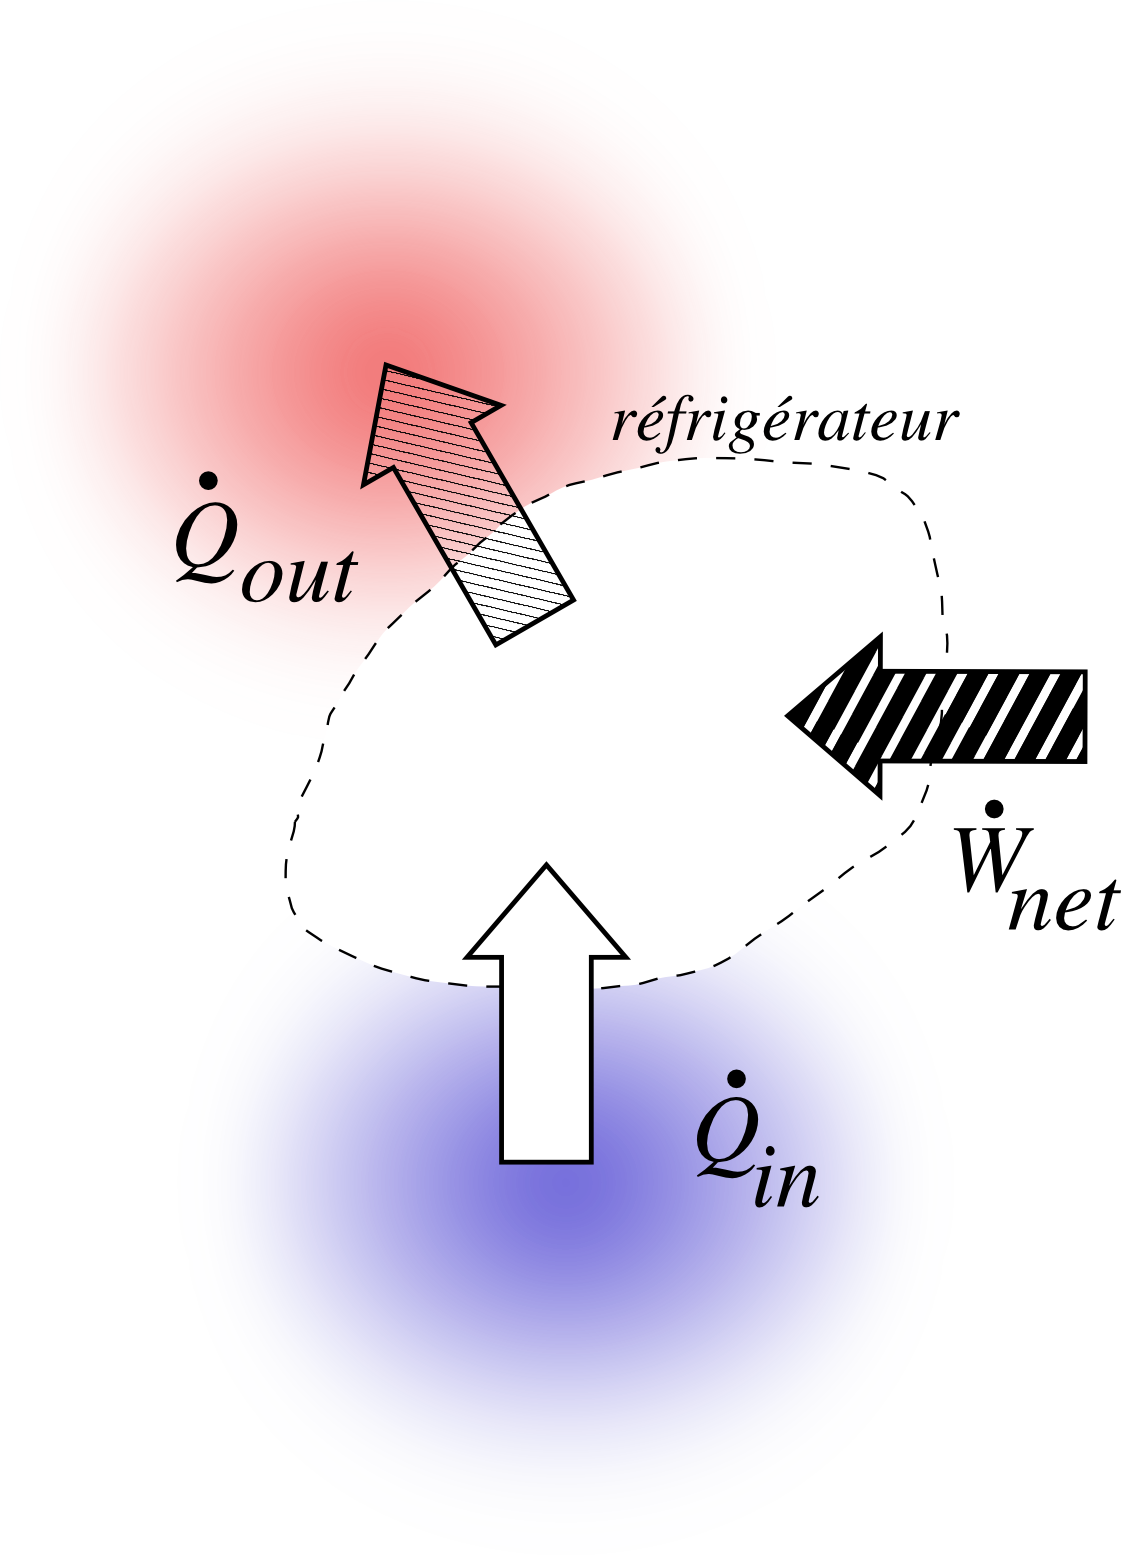
\includegraphics[height=10cm]{images/eff_refrigerateur.png}
				\end{center}
				\caption{Schématisation d’un réfrigérateur ou climatiseur.
			On souhaite obtenir un grand transfert $\dot{Q}_\text{in}$ (résultat) à partir du transfert $\dot{W}_\text{net}$ (coût).}
				\label{fig_transferts_réfrigérateur}
			\end{figure}

			D’après la définition~\ref{def_efficacité_machines_thermiques} le rendement (dit aussi parfois \vocab{coefficient of performance}, ou $COP_\text{réf.}$) d’un réfrigérateur ou d’un climatiseur est donc :
			\begin{equation}
				\eta_\text{réfrigérateur} = \eta _\text{climatiseur} \equiv  \left| \frac{\dot{Q}_\text{in}}{\dot{W}_\text{net}} \right|
			\end{equation}

			\begin{anexample}
			Un réfrigérateur consomme une puissance électrique de~\SI{100}{\watt} ; il extrait de la chaleur de la chambre froide avec une puissance de~\SI{120}{\watt}. Quel est son rendement ?
			
			\begin{answer}
				Le rendement est de $\eta_\text{réfrigérateur} = \left| \frac{\dot{Q}_\text{in}}{\dot{W}_\text{net}} \right| = \left| \frac{\num{+120}}{\num{+100}} \right| = \num{1,2} = \SI{120}{\percent}$. 
					\begin{remark} Ce réfrigérateur effectue un rejet $\dot{Q}_\text{out} = -\dot{W}_\text{net} - \dot{Q}_\text{in} = \num{-100} - \num{120}= \SI{-220}{\watt}$ à l’extérieur de la chambre froide (usuellement, dans l’habitation elle-même).\end{remark}
					\begin{remark} Les réfrigérateurs et climatiseurs domestiques ont souvent un rendement supérieur à~\num{1} mais en fonction des températures demandées, le rendement peut tout à fait y être inférieur.\end{remark}
			\end{answer}
		\end{anexample}

			En prenant garde aux pièges algébriques qu’amènent les valeurs absolues, pour préparer le chapitre prochain nous pouvons exprimer ce rendement en fonction des quantités de chaleur uniquement :
			\begin{equation}
				\eta _\text{réfrigérateur} = \eta _\text{climatiseur} = \frac{1}{\left| \frac{\dot{Q}_\text{out}}{\dot{Q}_\text{in}} \right| - 1}
				\label{rendement_réfrigérateur_qin_qout}
			\end{equation}





	\subsection{Rendement d’une pompe à chaleur}
	\label{ch_rendement_thermopompe}

		Une pompe à chaleur fonctionne exactement de la même manière qu’un climatiseur --\ il s’agit d’ailleurs souvent de la même machine\footnote{Une pompe à chaleur dite \vocab{réversible} devient facilement climatiseur --\ il suffit de retourner l’installation sur elle-même, ou d’inverser le sens de circulation du fluide. Attention, ces machines n’en sont pas pour autant réversibles au sens thermodynamique du terme, comme nous le verrons au \courssept.}\nolinebreak.
		Sa fonction est de générer un transfert $\dot{Q}_\text{out}$ vers la section «~chaude~» (usuellement l’intérieur d’une habitation). Ce transfert, représenté en \cref{fig_transferts_thermopompe} est rendu possible par l’apport à la thermopompe d’un travail, $\dot{W}_\text{net}$ , «~dépense~» nécessairement positive.

		\begin{figure}
			\begin{center}
				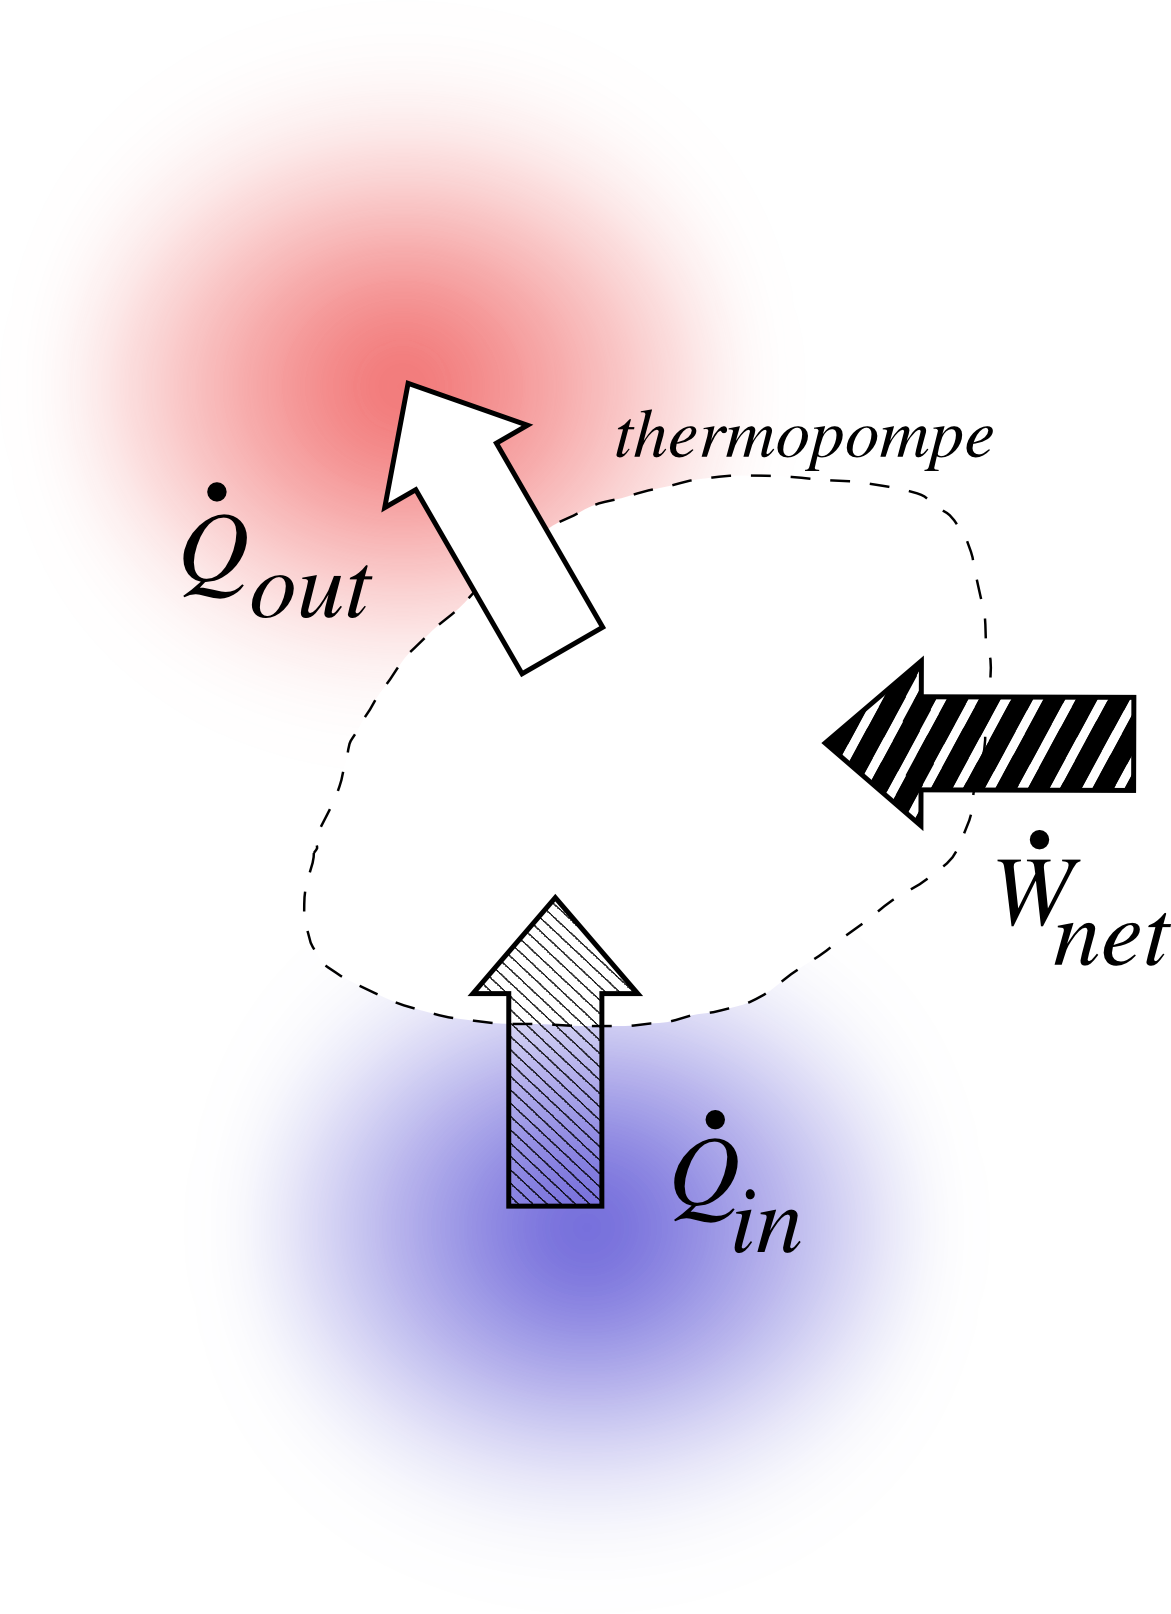
\includegraphics[height=10cm]{images/eff_thermopompe.png}
			\end{center}
			\caption{Schématisation d’une pompe à chaleur. On souhaite obtenir un grand transfert $\dot{Q}_\text{out}$ (résultat) à partir du transfert $\dot{W}_\text{net}$ (coût).}
			\label{fig_transferts_thermopompe}
		\end{figure}

		Le rendement (dit aussi \vocabe{coefficient of performance} ou $COP_{TP}$) de la thermopompe est donc défini par :
		\begin{equation}
			\eta_\text{thermopompe} \equiv  \left| \frac{\dot{Q}_\text{out}}{\dot{W}_\text{net}} \right|
			\label{def_rendement_thermopompe}
		\end{equation}
		
		\begin{anexample}
			Une pompe à chaleur consomme une puissance électrique de~\SI{100}{\watt} ; elle chauffe l’intérieur d’une pièce avec une puissance de~\SI{350}{\watt}. Quel est son rendement ?
			
			\begin{answer}
				Le rendement est de $\eta_\text{thermopompe} = \left| \frac{\dot{Q}_\text{out}}{\dot{W}_\text{net}} \right| = \left| \frac{\num{-350}}{\num{+100}} \right| = \num{3.5}$. 
					\begin{remark} La pompe à chaleur rejette plus de chaleur qu’elle ne consomme de travail –\ c’est tout son intérêt. Si le $COP$ était égal ou inférieur à~\num{1}, il serait plus économique et bien plus simple d’utiliser un radiateur électrique.\end{remark}
			\end{answer}
		\end{anexample}


		De la même façon que pour les sections précédentes, on peut exprimer ce rendement en fonction des débits de chaleur uniquement :
		\begin{equation}
			\eta_\text{thermopompe} = \frac{1}{1 - \left| \frac{\dot{Q}_\text{in}}{\dot{Q}_\text{out}} \right|}
			\label{eq_rendement_thermopompe_qin_qout}
		\end{equation}




	\subsection{De la faible performance des machines}

		Dans tous les cas que nous avons étudiés plus haut, pour chaque cycle, nous avons inclus un transfert indésirable. Dans le cycle moteur, une partie de l’énergie est gâchée sous forme de rejet de chaleur ($\dot{Q}_\text{out}$). Dans les cycles de réfrigération, on doit apporter du travail ($\dot{W}_\text{in}$).

		L’étudiant/e en ingénierie s’indignera inévitablement de la place accordée à ces pertes dans ce chapitre --\ et des timides rendements atteints par les machines décrites en exemple. Pourquoi les rendements calculés dans les exemples sont-ils si faibles, et surtout, comment concevoir des cycles de plus grande efficacité ? Nous aurons soin et à cœur de répondre à ces questions au \courssept.
